\scanpage{55}
Connaissant $v$ et $w$, on trouve donc \deleted{Donc} comme d'habitude qu'il existe un
\[
g\in G(\mathbb A_{\unsure{C|c}})=\prod_{\ell\ \mathrm{fini}}G(\mathbf Z_\ell)\times G(\mathbf C),
\]
tel que
\[
\deleted{\unsure{w=gv}}
\qquad M_w^{\deleted{\unsure{\mathbf Q}}\inserted{\mathbf Z}}=gM_v^{\deleted{\unsure{\mathbf Q}}\inserted{\mathbf Z}}
\]
où $G=G_{M\xi_v}$ est le grp alg. sur $\mathbf Q$ associé à $M,v$.

[\unsure{On vérifie|On considère} \unsure{que} les foncteurs $N\rightsquigarrow N_v^{\mathbf Z}$ et $N\rightsquigarrow N_w^{\mathbf Z}$ sur la catégorie des \uline{motifs} \uline{subordonnés} à $M$ sont isomorphes, \unsure{ce par considération par isomorphismes}]. D'ailleurs, $g$ est déterminé mod. multiplication à droite par $h\in G(\mathbf Z)$.
\inserted{$g\rightsquigarrow gh$ ($h\in G(\mathbf Z)$).}
\margin{N.B. Si on a fixé $g_\infty$ (ce qui est une indétermination mod $G(\mathbf Z)$ seulement) tous les $g_\ell$ sont déterminés.}

\deleted{Alors} On aura \inserted{\uline{en particulier}} pour $\sigma\in\operatorname{Gal}(k/k_0)$
\diagram{\begin{tikzcd}[ampersand replacement=\&,row sep=large]
\deleted{M_{\sigma w}^{\mathbf Z}=\dot\sigma(gM_v^{\mathbf Z})}\arrow[d]\\
M_{\sigma w}^{\mathbf Z}=\deleted{\unsure{g_\infty}}g_\sigma M_v^{\mathbf Z}\arrow[d,equal]\\
\sigma_\infty M_v^{\mathbf Z}
\end{tikzcd}}

\deleted{\margin{\figure{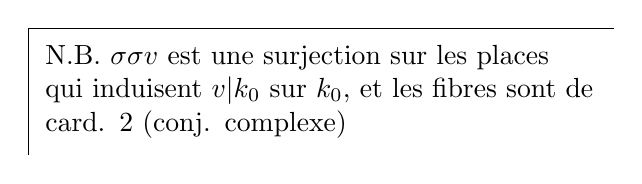
\begin{tikzpicture}
\node[align=left,text width=7cm,inner sep=6pt] (n) {N.B. $\sigma\rightsquigarrow\sigma v$ est une surjection sur les places qui induisent $v|k_0$ sur $k_0$, et les fibres sont de card. $2$ (conj. complexe)};
\draw (n.south west)--(n.north west)--(n.north east);
\end{tikzpicture}}}}
\deleted{donc on a une application
\diagram{\begin{tikzcd}[ampersand replacement=\&,column sep=large,execute at end picture={\draw ([xshift=-8pt,yshift=14pt]current bounding box.north west) rectangle ([xshift=8pt,yshift=-14pt]current bounding box.south east);}]
\operatorname{Gal}(k/k_0)\arrow[r,"\varphi_v"]\&G(\mathbb A_{\unsure{C|c}})/G(\mathbf Z)
\end{tikzcd}}
\[
M_{\sigma v}^{\mathbf Z}=\deleted{g_\sigma}\varphi_v(\sigma)M_v^{\mathbf Z}\quad\text{i.e.}\quad\dot\sigma_\infty(M_v^{\mathbf Z})=\varphi_v(\sigma)M_v^{\mathbf Z}
\]}
\mspage{54}
